% !TeX root = ../main.tex
% 原始章节：13-opration-system.Rmd

\chapter{操作系统移植}\label{chap:13-operating-system}

\section{运行操作系统所需要的支持}\label{sec:13-operating-system-001}

操作系统是直接运行在硬件上的一类特殊软件，可以进一步向用户软件提供支持服务和维护。

本文语境下的操作系统，指具有抢占式调度且支持页式内存管理的常见通用操作系统。
当我们的处理器对MMU、中断异常、时钟、MMIO 等硬件机制提供足够支持后，就具备了运行操作系统的基本硬件条件。之后需要做的就是完成操作系统对处理器的适配。
操作系统对处理器的适配具体来说，也就是对上面的几个硬件机制的适配融合。

操作系统软件借助 MMU 和异常完成页式内存管理，借助时钟和中断完成抢占式调度支持，借助 MMIO 实现交互和对更多硬件的控制。
操作系统移植，实际就是将操作系统的这些机能，具体实现到对应体系结构的硬件机制上。以下我们以教学操作系统 MOS 的移植为例，展示移植的具体过程。之后以 Linux 为例，介绍对驱动进行适配的板级移植。

\section{MOS 移植流程}\label{sec:13-operating-system-002}

\subsubsection{1. 为新的体系结构定义头文件定义}\label{sec:13-operating-system-003}

为新的体系结构准备体系结构相关的头文件。这些头文件通常包含通用寄存器定义，控制状态寄存器定义，页表属性定义，部分内联汇编函数定义等。

如下文件，定义了 LoongArch32 指令集中的所有通用寄存器别名以及控制状态寄存器。

% 代码语言：BookC
\begin{CodeBlock}[language=BookC]
#ifndef _SYS_REGDEF_H
#define _SYS_REGDEF_H

#define zero $r0
#define ra $r1
#define tp $r2
#define sp $r3
#define a0 $r4
#define a1 $r5
#define a2 $r6
#define a3 $r7
#define a4 $r8
#define a5 $r9
#define a6 $r10
#define a7 $r11
#define v0 $r10 // r4
#define v1 $r11 // r5
#define t0 $r12
#define t1 $r13
#define t2 $r14
#define t3 $r15
#define t4 $r16
#define t5 $r17
#define t6 $r18
#define t7 $r19
#define t8 $r20
#define x $r21
#define fp $r22
#define s0 $r23
#define s1 $r24
#define s2 $r25
#define s3 $r26
#define s4 $r27
#define s5 $r28
#define s6 $r29
#define s7 $r30
#define s8 $r31

#define csr_crmd 0x0
#define csr_prmd 0x1
#define csr_euen 0x2
#define csr_ectl 0x4
#define csr_estat 0x5
#define csr_era 0x6
#define csr_badv 0x7
#define csr_eentry 0xc
#define csr_tlbidx 0x10
#define csr_tlbehi 0x11
#define csr_tlbelo0 0x12
#define csr_tlbelo1 0x13
#define csr_asid 0x18
#define csr_pgdl 0x19
#define csr_pgdh 0x1a
#define csr_pgd 0x1b
#define csr_cpuid 0x20
#define csr_save0 0x30
#define csr_save1 0x31
#define csr_save2 0x32
#define csr_save3 0x33
#define csr_tid 0x40
#define csr_tcfg 0x41
#define csr_tval 0x42
#define csr_ticlr 0x44
#define csr_llbctl 0x60
#define csr_tlbrentry 0x88
#define csr_dmw0 0x180
#define csr_dmw1 0x181

#define ESTAT_SWI0 0x0001
#define ESTAT_SWI1 0x0002
#define ESTAT_HWI0 0x0004
#define ESTAT_HWI1 0x0008
#define ESTAT_HWI2 0x0010
#define ESTAT_HWI3 0x0020
#define ESTAT_HWI4 0x0040
#define ESTAT_HWI5 0x0080
#define ESTAT_HWI6 0x0100
#define ESTAT_HWI7 0x0200
#define ESTAT_TI 0x0800
#define ESTAT_IPI 0x1000

#define ESTAT_ECODE 0x003f0000
#define ESTAT_ESUBCODE 0x7fc00000

#define CRMD_PLV 0x0003
#define CRMD_IE 0x0004
#define CRMD_DA 0x0008
#define CRMD_PG 0x0010
#define CRMD_DATF 0x0020
#define CRMD_DATM 0x0080

#define PRMD_PPLV 0x0003
#define PRMD_PIE 0x0004

#endif /* _SYS_REGDEF_H */
\end{CodeBlock}

如下文件定义了缓存行的相关控制内联汇编函数：

% 代码语言：BookC
\begin{CodeBlock}[language=BookC]
#ifndef __ASM_CACHEOPS_H
#define __ASM_CACHEOPS_H

#ifndef __ASSEMBLY__

static inline void la_cache(int op, const volatile void *addr)
{
    __asm__ __volatile__("cacop %0, %1" : : "i"(op), "R" (*(unsigned char *)(addr)));
}

#define MIPS32_WHICH_ICACHE                    0x0
#define MIPS32_FETCH_AND_LOCK                  0x7

#define ICACHE_LOAD_LOCK (MIPS32_WHICH_ICACHE | (MIPS32_FETCH_AND_LOCK << 2))

/* Prefetch and lock instructions into cache */
static inline void icache_lock(void *func, size_t len)
{
}
#endif /* !__ASSEMBLY__ */

#define Cache_I             0x00
#define Cache_D             0x01
#define Cache_V             0x02
#define Cache_S             0x03

#define INDEX_INVALIDATE        0x08
#define INDEX_WRITEBACK_INV     0x08
#define HIT_INVALIDATE          0x10
#define HIT_WRITEBACK_INV       0x10

#define INDEX_INVALIDATE_I      (Cache_I | INDEX_INVALIDATE)
#define INDEX_WRITEBACK_INV_D   (Cache_D | INDEX_WRITEBACK_INV)
#define HIT_INVALIDATE_I        (Cache_I | HIT_INVALIDATE)
#define HIT_INVALIDATE_D        (Cache_D | HIT_INVALIDATE)
#define HIT_WRITEBACK_INV_D     (Cache_D | HIT_WRITEBACK_INV)

#endif  /* __ASM_CACHEOPS_H */

\end{CodeBlock}

如下文件定义了内核态下的虚拟内存布局，及虚拟地址相关的宏定义：

% 代码语言：BookC
\begin{CodeBlock}[language=BookC]
#ifndef _MMU_H_
#define _MMU_H_

#include <error.h>

#define PMEMSIZE (56 * 1024 * 1024)

#define NASID 1024
#define PAGE_SIZE 4096
#define PTMAP PAGE_SIZE
#define PDMAP (4 * 1024 * 1024) // bytes mapped by a page directory entry
#define PGSHIFT 12
#define PDSHIFT 22 // log2(PDMAP)
#define PDX(va) ((((u_long)(va)) >> PDSHIFT) & 0x03FF)
#define PTX(va) ((((u_long)(va)) >> PGSHIFT) & 0x03FF)
#define PTE_ADDR(pte) (((u_long)(pte)) & ~0xFFF)
#define PTE_FLAGS(pte) (((u_long)(pte)) & 0xFFF)

// Page number field of an address
#define PPN(pa) (((u_long)(pa)) >> PGSHIFT)
#define VPN(va) (((u_long)(va)) >> PGSHIFT)

// Global bit. When the G bit in a TLB entry is set, that TLB entry will match solely on the VPN
// field, regardless of whether the TLB entry’s ASID field matches the value in EntryHi.
#define PTE_G (0x0001 << (6 + 4))

// Valid bit. If 0 any address matching this entry will cause a tlb miss exception (TLBL/TLBS).
#define PTE_V (0x0001 << (0 + 4))

// Dirty bit, but really a write-enable bit. 1 to allow writes, 0 and any store using this
// translation will cause a tlb mod exception (TLB Mod).
#define PTE_D (0x0001 << (1 + 4))

// Permission bit.
#define PTE_PLV (0x0003 << (2 + 4))

// Cacheable bit. 1 to make the access cacheable, 0 for uncacheable.
#define PTE_C (0x0001 << (4 + 4))

// Copy On Write. Reserved for software, used by fork.
#define PTE_COW 0x0001

// Shared memmory. Reserved for software, used by fork.
#define PTE_LIBRARY 0x0002

// Memory segments (32-bit kernel mode addresses)
#define KUSEG 0x00000000U
#define KSEG0 0x80000000U
#define KSEG1 0xA0000000U
#define KSEG2 0xC0000000U

/*
 * Part 2.  Our conventions.
 */

/*
 o     4G ----------->  +----------------------------+------------0x100000000
 o                      |       ...                  |  kseg2
 o      KSEG2    -----> +----------------------------+------------0xc000 0000
 o                      |          Devices           |  kseg1
 o      KSEG1    -----> +----------------------------+------------0xa000 0000
 o                      |      Invalid Memory        |   /|\
 o                      +----------------------------+----|-------Physical Memory Max
 o                      |       ...                  |  kseg0
 o      KSTACKTOP-----> +----------------------------+----|-------0x8040 0000-------end
 o                      |       Kernel Stack         |    | KSTKSIZE            /|\
 o                      +----------------------------+----|------                |
 o                      |       Kernel Text          |    |                    PDMAP
 o      KERNBASE -----> +----------------------------+----|-------0x8002 0000    |
 o                      |      Exception Entry       |   \|/                    \|/
 o      ULIM     -----> +----------------------------+------------0x8000 0000-------
 o                      |         User VPT           |     PDMAP                /|\
 o      UVPT     -----> +----------------------------+------------0x7fc0 0000    |
 o                      |           pages            |     PDMAP                 |
 o      UPAGES   -----> +----------------------------+------------0x7f80 0000    |
 o                      |           envs             |     PDMAP                 |
 o  UTOP,UENVS   -----> +----------------------------+------------0x7f40 0000    |
 o  UXSTACKTOP -/       |     user exception stack   |     PTMAP                 |
 o                      +----------------------------+------------0x7f3f f000    |
 o                      |                            |     PTMAP                 |
 o      USTACKTOP ----> +----------------------------+------------0x7f3f e000    |
 o                      |     normal user stack      |     PTMAP                 |
 o                      +----------------------------+------------0x7f3f d000    |
 a                      |                            |                           |
 a                      ~~~~~~~~~~~~~~~~~~~~~~~~~~~~~~                           |
 a                      .                            .                           |
 a                      .                            .                         kuseg
 a                      .                            .                           |
 a                      |~~~~~~~~~~~~~~~~~~~~~~~~~~~~|                           |
 a                      |                            |                           |
 o       UTEXT   -----> +----------------------------+------------0x0040 0000    |
 o                      |      reserved for COW      |     PTMAP                 |
 o       UCOW    -----> +----------------------------+------------0x003f f000    |
 o                      |   reversed for temporary   |     PTMAP                 |
 o       UTEMP   -----> +----------------------------+------------0x003f e000    |
 o                      |       invalid memory       |                          \|/
 a     0 ------------>  +----------------------------+ ----------------------------
 o
*/

#define KERNBASE 0x80020000

#define KSTACKTOP (ULIM + PDMAP)
#define ULIM 0x80000000

#define UVPT (ULIM - PDMAP)
#define UPAGES (UVPT - PDMAP)
#define UENVS (UPAGES - PDMAP)

#define UTOP UENVS
#define UXSTACKTOP UTOP

#define USTACKTOP (UTOP - 2 * PTMAP)
#define UTEXT PDMAP
#define UCOW (UTEXT - PTMAP)
#define UTEMP (UCOW - PTMAP)

#ifndef __ASSEMBLER__

/*
 * Part 3.  Our helper functions.
 */
#include <error.h>
#include <string.h>
#include <types.h>

extern u_long npage;

typedef u_long Pde;
typedef u_long Pte;

// TODO: naming this struct
typedef struct {
    Pte entry[2];
} tlb_entry_t;

#define PADDR(kva)                                                                                 \
    ({                                                                                         \
        u_long _a = (u_long)(kva);                                                         \
        if (_a < ULIM)                                                                     \
            panic("PADDR called with invalid kva %08lx", _a);                          \
        _a - ULIM;                                                                         \
    })

// translates from physical address to kernel virtual address
#define KADDR(pa)                                                                                  \
    ({                                                                                         \
        u_long _ppn = PPN(pa);                                                             \
        if (_ppn >= npage) {                                                               \
            panic("KADDR called with invalid pa %08lx", (u_long)pa);                   \
        }                                                                                  \
        (pa) + ULIM;                                                                       \
    })

#define assert(x)                                                                                  \
    do {                                                                                       \
        if (!(x)) {                                                                        \
            panic("assertion failed: %s", #x);                                         \
        }                                                                                  \
    } while (0)

#define TRUP(_p)                                                                                   \
    ({                                                                                         \
        typeof((_p)) __m_p = (_p);                                                         \
        (u_int) __m_p > ULIM ? (typeof(_p))ULIM : __m_p;                                   \
    })

extern void tlb_out(u_int entryhi);
void tlb_invalidate(u_int asid, u_long va);
#endif //!__ASSEMBLER__
#endif // !_MMU_H_

\end{CodeBlock}

这一部分主要实现依据是体系结构手册，有一部分是机械性的将手册中表示的寄存器等信息直接 copy 过来。也有一部分是需要在理解手册的基础上，进行设计和实现，如虚拟地址相关的头文件。

体系结构手册中，并没有对内核态下的虚拟地址空间分配情况进行定义，手册中只是介绍了 LoongArch 处理器，进行虚拟地址翻译的整体流程机制。这里的虚拟地址空间分配，是人为在手册定义的虚拟地址翻译流程机制约束下定义出来的。这里的选择其实具有一定的任意性。如地址 ULIM，其实并没有体系结构机制，约束它一定定义在 0x8000\_0000 这个虚拟地址上，想定义在 0xc000\_0000 这个地址也没有问题。选择 0x8000\_0000 而不是 0xc000\_0000 更多就是一种人为的随机选择。体系结构实际上只是隐性约束了 ULIM 这个地址，一定需要是 512M 对齐的。相关约束也并没有显式的表示，实际上是通过体系结构中 DMW 寄存器（提供内核线性映射区域）参与的虚拟地址翻译流程带来的隐性约束。

在进行体系结构移植时，开发者需要对目标体系结构有详实的了解，以在体系结构移植过程中，满足这些``隐式''约束。

\subsubsection{2. 完成启动部分内核初始化代码}\label{sec:13-operating-system-004}

引导程序对处理器和平台完成一系列初始化工作后，会将处理器控制流转移到操作系统中。具体来说，是转移到操作系统的启动代码中。

启动代码接手引导程序完成基本初始化的硬件平台，并进一步为操作系统运行准备环境。如配置控制寄存器，使得处理器处于某种地址翻译状态，以符合先前头文件中对虚拟地址空间的定义。如配置栈指针，使得处理器可以运行后续 C 部分的代码。如抹除 BSS 段区域的数据，以提供正确的运行环境。完成一系列初始化操作后，启动代码将会跳转到由 C 语言编写的后续内核初始化代码。

% 代码语言：BookC
\begin{CodeBlock}[language=BookC]
#include <asm/asm.h>
#include <mmu.h>

.text
.globl  _start
_start:
    /* initialize */
    #if !defined(LAB) || LAB >= 3
    la      a0, exc_gen_entry
    csrwr   a0, csr_eentry
    #endif
    #if !defined(LAB) || LAB >= 2
    la      a1, tlb_miss_entry
    li.w    a0, 0x1fffffff
    and     a1, a1, a0
    csrwr   a1, csr_tlbrentry
    #endif

    /* disable interrupts and enable memory map */
    li.w    a0, 0xb0     // PLV = 0, ID = 0, DA = 0, PG = 1, DATF = DATM = 01
    csrwr   a0, csr_crmd

    /* set page size 2^12B=4KB for tlb */
    li.w    a0, 0x0c000000
    csrwr   a0, csr_tlbidx

    /* initialize timer */
    li.w    t0, ESTAT_TI
    csrwr   t0, csr_ectl

    /* ----- MOS EXERCISE 1 boot AFTER basic-lds BEGIN ----- */
    /* hint: you can refer to the memory layout in include/mmu.h */
    /* set up the kernel stack */
    // ----- MOS BLANK BEGIN -----
    li.w    sp, KSTACKTOP
    // ----- MOS BLANK END -----

    /* clear bss segment for C env. */
    la      t0, .bss
    la      t1, bss_end
bss_loop:
    beq     t0, t1, bss_loop_end
    st.b    zero, t0, 0
    addi.w  t0, t0, 1
    b       bss_loop
bss_loop_end:
    /* jump to la32r_init */
    // ----- MOS BLANK BEGIN -----
    b       la32r_init
    // ----- MOS BLANK END -----
    /* ----- MOS EXERCISE END ----- */
    nop

\end{CodeBlock}

启动部分一般使用汇编语言编写，同时涉及对控制寄存器的直接操作，因此是与体系结构密切相关的。

\subsubsection{3. 修改编译、链接脚本}\label{sec:13-operating-system-005}

完成上述操作后，需要适配修改编译和链接脚本，使得内核能够被正确编译并链接到正确的地址上。

内核正确编译链接后，即可通过 QEMU 等模拟器调试运行，查看内核执行情况是否符合预期。

% 代码语言：BookLoongArch
\begin{CodeBlock}[language=BookLoongArch]
/*
 * Set the architecture to loongarch32.
 */
OUTPUT_ARCH(loongarch32)

/*
 * Set the ENTRY point of the program to _start.
 */
ENTRY(_start)

SECTIONS {
    /* ----- MOS EXERCISE 3 exc-entry-lds AFTER exc-entry BEGIN ----- */
    /* ----- MOS BLANK BEGIN ----- */
    . = 0x80000000;
    .tlb_miss_entry : {
        *(.text.tlb_miss_entry)
    }

    . = 0x80000180;
    .exc_gen_entry : {
        *(.text.exc_gen_entry)
    }
    /* ----- MOS BLANK END ----- */
    /* ----- MOS EXERCISE END ----- */

    /* ----- MOS EXERCISE 1 basic-lds AFTER readelf BEGIN ----- */
    /* fill in the correct address of the key sections: text, data, bss. */
    /* Hint: The loading address can be found in the memory layout. And the data section
     *       and bss section are right after the text section, so you can just define
     *       them after the text section.
     */
    /* Step 1: Set the loading address of the text section to the location counter ".". */
    /* ----- MOS BLANK BEGIN ----- */
    . = 0x80020000;
    /* ----- MOS BLANK END ----- */

    /* Step 2: Define the text section. */
    /* ----- MOS BLANK BEGIN ----- */
    .text : {
        *(.text)
    }
    /* ----- MOS BLANK END ----- */

    /* Step 3: Define the data section. */
    /* ----- MOS BLANK BEGIN ----- */
    .data : {
        *(.data)
    }
    /* ----- MOS BLANK END ----- */

    bss_start = .;
    /* Step 4: Define the bss section. */
    /* ----- MOS BLANK BEGIN ----- */
    .bss  : {
        *(.bss)
    }
    /* ----- MOS BLANK END ----- */
    /* ----- MOS EXERCISE END ----- */

    bss_end = .;
    . = 0x80400000;
    end = . ;
}

\end{CodeBlock}

这里要与前文定义在头文件中的虚拟地址空间相匹配

\subsubsection{4. 适配串口驱动程序，允许内核打印输出}\label{sec:13-operating-system-006}

在上述实现正确完成之后，需要为新的硬件平台编写串口驱动程序，允许内核与外部进行输入输出的交互操作，也方便在内核中通过 printk 进行调试。这部分实际上与体系结构无较多关系，仅与硬件平台有关。

% 代码语言：BookC
\begin{CodeBlock}[language=BookC]
#include <megasoc.h>
#include <mmu.h>
#include <printk.h>

/* Overview:
 *   Send a character to the console. If Transmitter Holding Register is currently occupied by
 *   some data, wait until the register becomes available.
 *
 * Pre-Condition:
 *   'ch' is the character to be sent.
 */
void printcharc(char ch) {
    if (ch == '\n') {
        printcharc('\r');
    }
    while (!(*((volatile uint8_t *)(KSEG1 + MEGASOC_SERIAL_LSR)) & MEGASOC_SERIAL_THR_EMPTY)) {
    }
    *((volatile uint8_t *)(KSEG1 + MEGASOC_SERIAL_DATA)) = ch;
}

/* Overview:
 *   Read a character from the console.
 *
 * Post-Condition:
 *   If the input character data is ready, read and return the character.
 *   Otherwise, i.e. there's no input data available, 0 is returned immediately.
 */
int scancharc(void) {
    if (*((volatile uint8_t *)(KSEG1 + MEGASOC_SERIAL_LSR)) & MEGASOC_SERIAL_DATA_READY) {
        return *((volatile uint8_t *)(KSEG1 + MEGASOC_SERIAL_DATA));
    }
    return 0;
}

/* Overview:
 *   Halt/Reset the whole system. Write the magic value GORESET(0x42) to SOFTRES register of the
 *   FPGA on the MEGASOC board, initiating a board reset. In QEMU emulator, emulation will stop
 *   instead of rebooting with the parameter '-no-reboot'.
 *
 * Post-Condition:
 *   If the current device doesn't support such halt method, print a warning message and enter
 *   infinite loop.
 */
void halt(void) {
    // On QEMU
    *((u_int *)(KSEG1 + MEGASOC_FPGA_HALT_ADD)) = MEGASOC_FPGA_HALT_VAL;

    // On FPGA
    while (1) {
    }
}

\end{CodeBlock}

这里实现了最基础的轮询驱动，没有使用中断等硬件机制。

\subsubsection{5. 移植内存管理部分}\label{sec:13-operating-system-007}

虚拟地址翻译机制需要软硬件协同配合，也是与体系结构密切相关的。不同平台有不同的虚拟地址翻译机制。

操作系统一般对用户软件提供页式的虚拟地址翻译，但同为页式虚拟地址翻译，在不同体系结构下也有不同实现。

如 MMU 中的 TLB，就有软件重填与硬件重填两类。对于软件重填，页表结构完全可以由软件定义，较为灵活。对于硬件重填，页表结构则必须符合体系结构要求才行。

LoongArch 是一个类似 MIPS，采用软件重填的 TLB 构成 MMU 的体系结构。

具体移植中，首先是一部分汇编实现 TLB 重填，及 TLB 无效化的：

% 代码语言：BookLoongArch
\begin{CodeBlock}[language=BookLoongArch]
#include <asm/asm.h>
#include <mmu.h>

/* ----- MOS EXERCISE 2 tlb-invalidate AFTER page-insert BEGIN ----- */
LEAF(tlb_invalidate)
    /* Hint: Use invtlb 0x6 to invalidate page table entry. */
    // ----- MOS BLANK BEGIN -----
    invtlb  0x6, a0, a1
    // ----- MOS BLANK END -----
    jr      ra
END(tlb_invalidate)
/* ----- MOS EXERCISE END ----- */

/* ----- MOS EXERCISE 2 tlb-refill AFTER tlb-invalidate BEGIN ----- */
.section .text.tlb_miss_entry
.align 8
.global tlb_miss_entry
tlb_miss_entry:
    /* Step 1: Save general registers that we will use. */
    csrwr   t0, csr_save0
    csrwr   t1, csr_save1
    csrwr   t2, csr_save2
    /* Step 2: Get the corresponding page directory entry. */
    csrrd   t0, csr_pgd
    csrrd   t2, csr_badv
    srli.w  t1, t2, 20
    andi    t1, t1, 0xffc
    add.w   t1, t0, t1
    ld.w    t0, t1, 0
    /* Step 3: If the corresponding page table is not existent, */
    /* write an empty entry to TLB to trigger Page Invalid exception. */
    andi    t1, t0, PTE_V
    bne     t1, zero, 1f
    csrwr   zero, csr_tlbelo0
    csrwr   zero, csr_tlbelo1
    // Just use 'tlbfill' to write an empty entry to TLB
    // ----- MOS BLANK BEGIN -----
    tlbfill
    // ----- MOS BLANK END -----
    b       2f
1:
    /* Step 4: Get the corresponding page table entry, */
    /* and write to tlb. */
    li.w    t1, 0xfffff000
    and     t0, t0, t1
    srli.w  t1, t2, 10
    andi    t1, t1, 0xff8
    add.w   t1, t0, t1
    ld.w    t0, t1, 0
    ld.w    t2, t1, 4
    srli.w  t0, t0, 4
    srli.w  t2, t2, 4
    csrwr   t0, csr_tlbelo0
    csrwr   t2, csr_tlbelo1
    // Just use 'tlbfill' to write the corresponding page table entry to TLB
    // ----- MOS BLANK BEGIN -----
    tlbfill
    // ----- MOS BLANK END -----
2:
    /* Step 5: Restore general registers and return from excption. */
    csrrd   t2, csr_save2
    csrrd   t1, csr_save1
    csrrd   t0, csr_save0
    ertn
/* ----- MOS EXERCISE END ----- */

\end{CodeBlock}

TLB 无效化及 TLB 重填支持的机制，在不同体系结构下不同，反应到代码上也是有不同的实现。

之后针对上层页表部分抽象，也需要根据体系结构进行一些微调，如不同的权限位：

% 代码语言：BookDiff
\begin{CodeBlock}[language=BookDiff]
diff --git a/kern/pmap.c b/kern/pmap.c
index e62871f..c06a5dd 100644
--- a/kern/pmap.c
+++ b/kern/pmap.c
@@ -1,11 +1,10 @@
 #include <bitops.h>
 #include <env.h>
-#include <malta.h>
 #include <mmu.h>
 #include <pmap.h>
 #include <printk.h>
 
-/* These variables are set by mips_detect_memory(ram_low_size); */
+/* These variables are set by la32r_detect_memory() */
 static u_long memsize; /* Maximum physical address */
 u_long npage;         /* Amount of memory(in pages) */
 
@@ -17,13 +16,13 @@ static u_long freemem;
 struct Page_list page_free_list; /* Free list of physical pages */
 
 /* Overview:
- *   Use '_memsize' from bootloader to initialize 'memsize' and
+ *   Use the 'PMEMSIZE' macro to initialize 'memsize' and
  *   calculate the corresponding 'npage' value.
  */
 /* ----- MOS EXERCISE 2 detect-mem BEGIN ----- */
-void mips_detect_memory(u_int _memsize) {
+void la32r_detect_memory() {
    /* Step 1: Initialize memsize. */
-   memsize = _memsize;
+   memsize = PMEMSIZE;
 
    /* Step 2: Calculate the corresponding 'npage' value. */
    // ----- MOS BLANK BEGIN -----
@@ -34,7 +33,6 @@ void mips_detect_memory(u_int _memsize) {
 }
 /* ----- MOS EXERCISE END ----- */
 
-/* ----- MOS KEY-CODE 2 alloc BEGIN ----- */
 /* Overview:
     Allocate `n` bytes physical memory with alignment `align`, if `clear` is set, clear the
     allocated memory.
@@ -71,20 +69,19 @@ void *alloc(u_int n, u_int align, int clear) {
    /* Step 5: return allocated chunk. */
    return (void *)alloced_mem;
 }
-/* ----- MOS KEY-CODE END ----- */
 
 /* Overview:
     Set up two-level page table.
    Hint:
     You can get more details about `UPAGES` and `UENVS` in include/mmu.h. */
-void mips_vm_init() {
+void la32r_vm_init() {
    /* Allocate proper size of physical memory for global array `pages`,
     * for physical memory management. Then, map virtual address `UPAGES` to
     * physical address `pages` allocated before. For consideration of alignment,
     * you should round up the memory size before map. */
    pages = (struct Page *)alloc(npage * sizeof(struct Page), PAGE_SIZE, 1);
    printk("to memory %x for struct Pages.\n", freemem);
-   printk("pmap.c:\t mips vm init success\n");
+   printk("pmap.c: la32r vm init success\n");
 }
 
 /* Overview:
@@ -206,9 +203,9 @@ static int pgdir_walk(Pde *pgdir, u_long va, int create, Pte **ppte) {
    // ----- MOS BLANK END -----
 
    /* Step 2: If the corresponding page table is not existent (valid) then:
-    *   * If parameter `create` is set, create one. Set the permission bits 'PTE_C_CACHEABLE |
-    *     PTE_V' for this new page in the page directory. If failed to allocate a new page (out
-    *     of memory), return the error.
+    *   * If parameter `create` is set, create one. Set the permission bits 'PTE_V | PTE_D |
+    *      PTE_C | PTE_PLV' for this new page in the page directory.
+    *      If failed to allocate a new page (out of memory), return the error.
     *   * Otherwise, assign NULL to '*ppte' and return 0.
     */
    // ----- MOS BLANK BEGIN -----
@@ -216,7 +213,7 @@ static int pgdir_walk(Pde *pgdir, u_long va, int create, Pte **ppte) {
        if (create) {
            try(page_alloc(&pp));
            *pgdir_entryp = page2pa(pp);
-           *pgdir_entryp = (*pgdir_entryp) | PTE_C_CACHEABLE | PTE_V;
+           *pgdir_entryp = (*pgdir_entryp) | PTE_V | PTE_D | PTE_C | PTE_PLV;
            pp->pp_ref++;
        } else {
            *ppte = 0;
@@ -236,7 +233,7 @@ static int pgdir_walk(Pde *pgdir, u_long va, int create, Pte **ppte) {
 
 /* Overview:
  *   Map the physical page 'pp' at virtual address 'va'. The permission (the low 12 bits) of the
- *   page table entry should be set to 'perm | PTE_C_CACHEABLE | PTE_V'.
+ *   page table entry should be set to 'perm | PTE_C | PTE_V'.
  *
  * Post-Condition:
  *   Return 0 on success
@@ -258,7 +255,7 @@ int page_insert(Pde *pgdir, u_int asid, struct Page *pp, u_long va, u_int perm)
            page_remove(pgdir, asid, va);
        } else {
            tlb_invalidate(asid, va);
-           *pte = page2pa(pp) | perm | PTE_C_CACHEABLE | PTE_V;
+           *pte = page2pa(pp) | perm | PTE_V | PTE_PLV | PTE_C;
            return 0;
        }
    }
@@ -274,10 +271,10 @@ int page_insert(Pde *pgdir, u_int asid, struct Page *pp, u_long va, u_int perm)
    try(pgdir_walk(pgdir, va, 1, &pte));
    // ----- MOS BLANK END -----
 
-   /* Step 4: Insert the page to the page table entry with 'perm | PTE_C_CACHEABLE | PTE_V'
+   /* Step 4: Insert the page to the page table entry with 'perm | PTE_V | PTE_PLV | PTE_C'
     * and increase its 'pp_ref'. */
    // ----- MOS BLANK BEGIN -----
-   *pte = page2pa(pp) | perm | PTE_C_CACHEABLE | PTE_V;
+   *pte = page2pa(pp) | perm | PTE_V | PTE_PLV | PTE_C;
    pp->pp_ref++;
    // ----- MOS BLANK END -----
 
@@ -285,7 +282,6 @@ int page_insert(Pde *pgdir, u_int asid, struct Page *pp, u_long va, u_int perm)
 }
 /* ----- MOS EXERCISE END ----- */
 
-/* ----- MOS KEY-CODE 2 page_lookup AFTER alloc BEGIN ----- */
 /*Overview:
     Look up the Page that virtual address `va` map to.
   Post-Condition:
@@ -312,7 +308,6 @@ struct Page *page_lookup(Pde *pgdir, u_long va, Pte **ppte) {
 
    return pp;
 }
-/* ----- MOS KEY-CODE END ----- */
 
 /* Overview:
  *   Decrease the 'pp_ref' value of Page 'pp'.
@@ -327,7 +322,6 @@ void page_decref(struct Page *pp) {
    }
 }
 
-/* ----- MOS KEY-CODE 2 page_remove AFTER page_lookup BEGIN ----- */
 // Overview:
 //   Unmap the physical page at virtual address 'va'.
 void page_remove(Pde *pgdir, u_int asid, u_long va) {
@@ -347,7 +341,6 @@ void page_remove(Pde *pgdir, u_int asid, u_long va) {
    tlb_invalidate(asid, va);
    return;
 }
-/* ----- MOS KEY-CODE END ----- */
 
 void physical_memory_manage_check(void) {
    struct Page *pp, *pp0, *pp1, *pp2;
@@ -466,9 +459,9 @@ void page_check(void) {
    // free pp0 and try again: pp0 should be used for page table
    page_free(pp0);
    assert(page_insert(boot_pgdir, 0, pp1, 0x0, 0) == 0);
-   assert(PTE_FLAGS(boot_pgdir[0]) == (PTE_C_CACHEABLE | PTE_V));
+   assert(PTE_FLAGS(boot_pgdir[0]) == (PTE_C | PTE_V | PTE_D | PTE_PLV));
    assert(PTE_ADDR(boot_pgdir[0]) == page2pa(pp0));
-   assert(PTE_FLAGS(*(Pte *)page2kva(pp0)) == (PTE_C_CACHEABLE | PTE_V));
+   assert(PTE_FLAGS(*(Pte *)page2kva(pp0)) == (PTE_C | PTE_V | PTE_PLV));
 
    printk("va2pa(boot_pgdir, 0x0) is %x\n", va2pa(boot_pgdir, 0x0));
    printk("page2pa(pp1) is %x\n", page2pa(pp1));
\end{CodeBlock}

\subsubsection{6. 实现中断异常支持}\label{sec:13-operating-system-008}

中断异常实现机制也是体系结构相关的，移植时，需要为新的体系结构准备新的中断异常处理代码，并适配相应处理的流程。

首先完成异常中断入口的实现，这里需要支持上下文的保存。这里还需要与体系结构硬件配合，完成对嵌套异常的支持。

% 代码语言：BookC
\begin{CodeBlock}[language=BookC]
#ifndef _TRAP_H_
#define _TRAP_H_

#ifndef __ASSEMBLER__

#include <types.h>

struct Trapframe {
    /* Saved main processor registers. */
    unsigned long regs[32];

    /* Saved special registers. */
    unsigned long crmd;
    unsigned long badv;
    unsigned long estat;
    unsigned long era;
};

void print_tf(struct Trapframe *tf);

#endif /* !__ASSEMBLER__ */

/*
 * Stack layout for all exceptions
 */

#define TF_REG0 0
#define TF_REG1 ((TF_REG0) + 4)
#define TF_REG2 ((TF_REG1) + 4)
#define TF_REG3 ((TF_REG2) + 4)
#define TF_REG4 ((TF_REG3) + 4)
#define TF_REG5 ((TF_REG4) + 4)
#define TF_REG6 ((TF_REG5) + 4)
#define TF_REG7 ((TF_REG6) + 4)
#define TF_REG8 ((TF_REG7) + 4)
#define TF_REG9 ((TF_REG8) + 4)
#define TF_REG10 ((TF_REG9) + 4)
#define TF_REG11 ((TF_REG10) + 4)
#define TF_REG12 ((TF_REG11) + 4)
#define TF_REG13 ((TF_REG12) + 4)
#define TF_REG14 ((TF_REG13) + 4)
#define TF_REG15 ((TF_REG14) + 4)
#define TF_REG16 ((TF_REG15) + 4)
#define TF_REG17 ((TF_REG16) + 4)
#define TF_REG18 ((TF_REG17) + 4)
#define TF_REG19 ((TF_REG18) + 4)
#define TF_REG20 ((TF_REG19) + 4)
#define TF_REG21 ((TF_REG20) + 4)
#define TF_REG22 ((TF_REG21) + 4)
#define TF_REG23 ((TF_REG22) + 4)
#define TF_REG24 ((TF_REG23) + 4)
#define TF_REG25 ((TF_REG24) + 4)
/*
 * $26 (k0) and $27 (k1) not saved
 */
#define TF_REG26 ((TF_REG25) + 4)
#define TF_REG27 ((TF_REG26) + 4)
#define TF_REG28 ((TF_REG27) + 4)
#define TF_REG29 ((TF_REG28) + 4)
#define TF_REG30 ((TF_REG29) + 4)
#define TF_REG31 ((TF_REG30) + 4)

#define TF_CRMD ((TF_REG31) + 4)

#define TF_BADV ((TF_CRMD) + 4)
#define TF_ESTAT ((TF_BADV) + 4)
#define TF_ERA ((TF_ESTAT) + 4)
/*
 * Size of stack frame, word/double word alignment
 */
#define TF_SIZE ((TF_ERA) + 4)
#endif /* _TRAP_H_ */

\end{CodeBlock}

% 代码语言：BookLoongArch
\begin{CodeBlock}[language=BookLoongArch]
#include <asm/asm.h>
#include <mmu.h>
#include <trap.h>

// clang-format off
.macro SAVE_ALL
    csrrd   x, csr_prmd
    andi    x, x, 0x3
    beq     x, zero, 1f
    move    x, sp
    li.w    sp, (KSTACKTOP - TF_SIZE)
    st.w    x, sp, TF_REG3
    b       2f
1:
    li.w    x, TF_SIZE
    st.w    sp, sp, TF_REG3 - TF_SIZE
    sub.w   sp, sp, x
2:
    csrrd   x, csr_prmd
    st.w    x, sp, TF_CRMD
    csrrd   x, csr_estat
    st.w    x, sp, TF_ESTAT
    csrrd   x, csr_era
    st.w    x, sp, TF_ERA
    csrrd   x, csr_badv
    st.w    x, sp, TF_BADV
    st.w    $r0, sp, TF_REG0
    st.w    $r1, sp, TF_REG1
    st.w    $r2, sp, TF_REG2
    st.w    $r4, sp, TF_REG4
    st.w    $r5, sp, TF_REG5
    st.w    $r6, sp, TF_REG6
    st.w    $r7, sp, TF_REG7
    st.w    $r8, sp, TF_REG8
    st.w    $r9, sp, TF_REG9
    st.w    $r10, sp, TF_REG10
    st.w    $r11, sp, TF_REG11
    st.w    $r12, sp, TF_REG12
    st.w    $r13, sp, TF_REG13
    st.w    $r14, sp, TF_REG14
    st.w    $r15, sp, TF_REG15
    st.w    $r16, sp, TF_REG16
    st.w    $r17, sp, TF_REG17
    st.w    $r18, sp, TF_REG18
    st.w    $r19, sp, TF_REG19
    st.w    $r20, sp, TF_REG20
    st.w    $r21, sp, TF_REG21
    st.w    $r22, sp, TF_REG22
    st.w    $r23, sp, TF_REG23
    st.w    $r24, sp, TF_REG24
    st.w    $r25, sp, TF_REG25
    st.w    $r26, sp, TF_REG26
    st.w    $r27, sp, TF_REG27
    st.w    $r28, sp, TF_REG28
    st.w    $r29, sp, TF_REG29
    st.w    $r30, sp, TF_REG30
    st.w    $r31, sp, TF_REG31
.endm
/*
 * Note that we restore the IE flags from stack. This means
 * that a modified IE mask will be nullified.
 */
.macro RESTORE_SOME
    ld.w    v0, sp, TF_CRMD
    csrwr   v0, csr_prmd
    ld.w    v1, sp, TF_ERA
    csrwr   v1, csr_era
    ld.w    $r31, sp, TF_REG31
    ld.w    $r30, sp, TF_REG30
    ld.w    $r29, sp, TF_REG29
    ld.w    $r28, sp, TF_REG28
    ld.w    $r27, sp, TF_REG27
    ld.w    $r26, sp, TF_REG26
    ld.w    $r25, sp, TF_REG25
    ld.w    $r24, sp, TF_REG24
    ld.w    $r23, sp, TF_REG23
    ld.w    $r22, sp, TF_REG22
    ld.w    $r21, sp, TF_REG21
    ld.w    $r20, sp, TF_REG20
    ld.w    $r19, sp, TF_REG19
    ld.w    $r18, sp, TF_REG18
    ld.w    $r17, sp, TF_REG17
    ld.w    $r16, sp, TF_REG16
    ld.w    $r15, sp, TF_REG15
    ld.w    $r14, sp, TF_REG14
    ld.w    $r13, sp, TF_REG13
    ld.w    $r12, sp, TF_REG12
    ld.w    $r11, sp, TF_REG11
    ld.w    $r10, sp, TF_REG10
    ld.w    $r9, sp, TF_REG9
    ld.w    $r8, sp, TF_REG8
    ld.w    $r7, sp, TF_REG7
    ld.w    $r6, sp, TF_REG6
    ld.w    $r5, sp, TF_REG5
    ld.w    $r4, sp, TF_REG4
    ld.w    $r2, sp, TF_REG2
    ld.w    $r1, sp, TF_REG1
.endm

\end{CodeBlock}

% 代码语言：BookLoongArch
\begin{CodeBlock}[language=BookLoongArch]
#include <asm/asm.h>
#include <stackframe.h>

.macro BUILD_HANDLER exception handler
LEAF(handle_\exception)
    move    a0, sp
    bl      \handler
    b       ret_from_exception
END(handle_\exception)
.endm

.text;
.globl ret_from_exception;                                                                             \
.align 3;
.type ret_from_exception, @function;
ret_from_exception:
    RESTORE_SOME
    ld.w    sp, sp, TF_REG3 /* Deallocate stack */
    ertn

LEAF(handle_int)
    csrrd   t0, csr_estat
    andi    t1, t0, ESTAT_TI
    bne     t1, zero, timer_irq
timer_irq:
    li.w    t0, 1
    csrwr   t0, csr_ticlr
    li.w    a0, 0
    b       schedule
END(handle_int)

BUILD_HANDLER tlb do_tlb_invalid

#if !defined(LAB) || LAB >= 4
BUILD_HANDLER mod do_tlb_mod
BUILD_HANDLER sys do_syscall
#endif

BUILD_HANDLER reserved do_reserved

\end{CodeBlock}

对于异常的处理，不同体系结构定义有不同的异常，这里需要针对体系结构编写对应异常处理的代码。

% 代码语言：BookC
\begin{CodeBlock}[language=BookC]
#include <env.h>
#include <pmap.h>
#include <printk.h>
#include <trap.h>

extern void handle_int(void);
extern void handle_tlb(void);
extern void handle_sys(void);
extern void handle_mod(void);
extern void handle_reserved(void);

void (*exception_handlers[64])(void) = {
    [0 ... 63] = handle_reserved, [0] = handle_int,   [1 ... 3] = handle_tlb,
#if !defined(LAB) || LAB >= 4
    [0x4] = handle_mod,       [0xb] = handle_sys,
#endif
};

/* Overview:
 *   The fallback handler when an unknown exception code is encountered.
 *   'genex.S' wraps this function in 'handle_reserved'.
 */
void do_reserved(struct Trapframe *tf) {
    print_tf(tf);
    u_int badva;
    u_int exc_code = (tf->estat >> 16) & 0x3f;
    if (exc_code == 0xd) {
        asm("csrrd %0, 0x7" : "=r"(badva) :);
        printk("Unknown inst is 0x%08x\n", *((u_int *)badva));
    }
    panic("Unknown ExcCode %x", exc_code);
}
#include <bitops.h>
#include <env.h>
#include <pmap.h>

static void passive_alloc(u_int va, Pde *pgdir, u_int asid) {
    struct Page *p = NULL;

    if (va < UTEMP) {
        panic("address too low");
    }

    if (va >= USTACKTOP && va < USTACKTOP + PAGE_SIZE) {
        panic("invalid memory");
    }

    if (va >= UENVS && va < UPAGES) {
        panic("envs zone");
    }

    if (va >= UPAGES && va < UVPT) {
        panic("pages zone");
    }

    if (va >= ULIM) {
        panic("kernel address");
    }

    panic_on(page_alloc(&p));
    panic_on(page_insert(pgdir, asid, p, PTE_ADDR(va), (va >= UVPT && va < ULIM) ? 0 : PTE_D));
}

/* Overview:
 *  Handle invalid page table entry.
 */
/* ----- MOS EXERCISE 2 c-do-tlb-invalid AFTER tlb-refill BEGIN ----- */
void do_tlb_invalid(struct Trapframe *tf) {
    u_int va, asid;
    Pte *ppte;

    va = tf->badv;
#if !defined(LAB) || LAB >= 3
    asid = curenv->env_asid;
#else
    asid = 0;
#endif
    tlb_invalidate(asid, va);
    /* Hints:
     *  Invoke 'page_lookup' repeatedly in a loop to find the page table entry 'pte' associated
     *  with the virtual address 'va' in the current address space 'cur_pgdir'.
     *
     *  **While** 'page_lookup' returns 'NULL', indicating that the 'pte' could not be found,
     *  allocate a new page using 'passive_alloc' until 'page_lookup' succeeds.
     */

    // ----- MOS BLANK BEGIN -----
    while (page_lookup(cur_pgdir, va, &ppte) == NULL) {
        passive_alloc(va, cur_pgdir, asid);
    }
    // ----- MOS BLANK END -----
}
/* ----- MOS EXERCISE END ----- */

#if !defined(LAB) || LAB >= 4
/* Overview:
 *   This is the TLB Mod exception handler in kernel.
 *   Our kernel allows user programs to handle TLB Mod exception in user mode, so we copy its
 *   context 'tf' into UXSTACK and modify the EPC to the registered user exception entry.
 *
 * Hints:
 *   'env_user_tlb_mod_entry' is the user space entry registered using
 *   'sys_set_user_tlb_mod_entry'.
 *
 *   The user entry should handle this TLB Mod exception and restore the context.
 */
/* ----- MOS EXERCISE 4 mod-handler AFTER duppage BEGIN ----- */
void do_tlb_mod(struct Trapframe *tf) {
    struct Trapframe tmp_tf = *tf;

    if (tf->regs[3] < USTACKTOP || tf->regs[3] >= UXSTACKTOP) {
        tf->regs[3] = UXSTACKTOP;
    }
    tf->regs[3] -= sizeof(struct Trapframe);
    *(struct Trapframe *)tf->regs[3] = tmp_tf;

    if (curenv->env_user_tlb_mod_entry) {
        tf->regs[4] = tf->regs[3];
        tf->regs[3] -= sizeof(tf->regs[4]);
        // Hint: Set 'cp0_epc' in the context 'tf' to 'curenv->env_user_tlb_mod_entry'.
        // ----- MOS BLANK BEGIN -----
        tf->era = curenv->env_user_tlb_mod_entry;
        // ----- MOS BLANK END -----
    } else {
        panic("TLB Mod but no user handler registered");
    }
}
/* ----- MOS EXERCISE END ----- */
#endif

\end{CodeBlock}

\subsubsection{7. 系统调用}\label{sec:13-operating-system-009}

绝大部分系统调用是体系结构无关的，但有一部分系统调用则与体系结构相关。这里需要针对新的体系结构，对一些依赖体系结构实现的系统调用进行更新。

% 代码语言：BookC
\begin{CodeBlock}[language=BookC]
diff --git a/kern/syscall_all.c b/kern/syscall_all.c
index 5371a5a..2dec783 100644
--- a/kern/syscall_all.c
+++ b/kern/syscall_all.c
@@ -81,7 +81,7 @@ int sys_env_destroy(u_int envid) {
    struct Env *e;
    try(envid2env(envid, &e, 1));
 
-   printk("[%08x] destroying %08x\n", curenv->env_id, e->env_id);
+   // printk("[%08x] destroying %08x\n", curenv->env_id, e->env_id);
    env_destroy(e);
    return 0;
 }
@@ -284,11 +284,7 @@ int sys_exofork(void) {
 
    /* Step 3: Set the new env's 'env_tf.regs[2]' to 0 to indicate the return value in child. */
    // ----- MOS BLANK BEGIN -----
-   e->env_tf.regs[2] = 0;
-   // ----- MOS BLANK END -----
-
-   /* Step 4: Set up the new env's 'env_status' and 'env_pri'.  */
-   // ----- MOS BLANK BEGIN -----
+   e->env_tf.regs[4] = 0;
    e->env_status = ENV_NOT_RUNNABLE;
    e->env_pri = curenv->env_pri;
    // ----- MOS BLANK END -----
@@ -360,7 +356,7 @@ int sys_set_trapframe(u_int envid, struct Trapframe *tf) {
        *((struct Trapframe *)KSTACKTOP - 1) = *tf;
        // return `tf->regs[2]` instead of 0, because return value overrides regs[2] on
        // current trapframe.
-       return tf->regs[2];
+       return tf->regs[4];
    } else {
        env->env_tf = *tf;
        return 0;
@@ -409,8 +405,7 @@ int sys_ipc_recv(u_int dstva) {
    TAILQ_REMOVE(&env_sched_list, curenv, env_sched_link);
    // ----- MOS BLANK END -----
 
-   /* Step 5: Give up the CPU and block until a message is received. */
-   ((struct Trapframe *)KSTACKTOP - 1)->regs[2] = 0;
+   ((struct Trapframe *)KSTACKTOP - 1)->regs[4] = 0;
    schedule(1);
 }
 
@@ -525,9 +520,9 @@ int sys_cgetc(void) {
  * * ---------------------------------*
  */
 // ----- MOS BLANK BEGIN ----- quiet
-int valid_addr_space_num = 2;
-unsigned int valid_addr_start[2] = {0x180003f8, 0x180001f0};
-unsigned int valid_addr_end[2] = {0x180003f8 + 0x20, 0x180001f8};
+#define VALID_ADDR_SPACE_NUM 2
+unsigned int valid_addr_start[VALID_ADDR_SPACE_NUM] = {0x180001f0, 0x1fe001e0};
+unsigned int valid_addr_end[VALID_ADDR_SPACE_NUM] = {0x180001f8, 0x1fe001e0 + 0x8};
 
 static inline int is_illegal_dev_range(u_long pa, u_long len) {
    if ((pa % 4 != 0 && len != 1 && len != 2) || (pa % 2 != 0 && len != 1)) {
@@ -536,7 +531,7 @@ static inline int is_illegal_dev_range(u_long pa, u_long len) {
    int i;
    u_int target_start = pa;
    u_int target_end = pa + len;
-   for (i = 0; i < valid_addr_space_num; i++) {
+   for (i = 0; i < VALID_ADDR_SPACE_NUM; i++) {
        if (target_start >= valid_addr_start[i] && target_end <= valid_addr_end[i]) {
            return 0;
        }
@@ -546,7 +541,7 @@ static inline int is_illegal_dev_range(u_long pa, u_long len) {
 // ----- MOS BLANK END -----
 int sys_write_dev(u_int va, u_int pa, u_int len) {
    // ----- MOS BLANK BEGIN -----
-   if (is_illegal_va_range(va, len) || is_illegal_dev_range(pa, len) || va % len != 0) {
+   if (is_illegal_va_range(va, len) || is_illegal_dev_range(pa, len) || va % 4 != 0) {
        return -E_INVAL;
    }
    if (len == 4) {
@@ -579,7 +574,7 @@ int sys_write_dev(u_int va, u_int pa, u_int len) {
  */
 int sys_read_dev(u_int va, u_int pa, u_int len) {
    // ----- MOS BLANK BEGIN -----
-   if (is_illegal_va_range(va, len) || is_illegal_dev_range(pa, len) || va % len != 0) {
+   if (is_illegal_va_range(va, len) || is_illegal_dev_range(pa, len) || va % 4 != 0) {
        return -E_INVAL;
    }
    if (len == 4) {
@@ -596,6 +591,20 @@ int sys_read_dev(u_int va, u_int pa, u_int len) {
 }
 /* ----- MOS EXERCISE END ----- */
 
+int sys_read_block(u_int secno, void *dst) {
+   // void* kva = (void*) KADDR(va2pa(curenv->env_pgdir, (u_long)dst));
+   memcpy(dst, (void *)0x83800000 + (secno * 512), 512);
+   // mmc_read_blocks(pdst, secno + 2099200, 1);
+   return 0;
+}
+
+int sys_write_block(u_int secno, const void *src) {
+   // void* kva = (void*) KADDR(va2pa(curenv->env_pgdir, (u_long)src));
+   memcpy((void *)0x83800000 + (secno * 512), src, 512);
+   // mmc_write_blocks(secno + 2099200, 1, psrc);
+   return 0;
+}
+
 void *syscall_table[MAX_SYSNO] = {
     [SYS_putchar] = sys_putchar,
     [SYS_print_cons] = sys_print_cons,
@@ -615,6 +624,8 @@ void *syscall_table[MAX_SYSNO] = {
     [SYS_cgetc] = sys_cgetc,
     [SYS_write_dev] = sys_write_dev,
     [SYS_read_dev] = sys_read_dev,
+    [SYS_read_block] = sys_read_block,
+    [SYS_write_block] = sys_write_block,
 };
 
 /* Overview:
@@ -632,13 +643,13 @@ void do_syscall(struct Trapframe *tf) {
    int (*func)(u_int, u_int, u_int, u_int, u_int);
    int sysno = tf->regs[4];
    if (sysno < 0 || sysno >= MAX_SYSNO) {
-       tf->regs[2] = -E_NO_SYS;
+       tf->regs[4] = -E_NO_SYS;
        return;
    }
 
    /* Step 1: Add the EPC in 'tf' by a word (size of an instruction). */
    // ----- MOS BLANK BEGIN -----
-   tf->cp0_epc += 4;
+   tf->era += 4;
    // ----- MOS BLANK END -----
 
    /* Step 2: Use 'sysno' to get 'func' from 'syscall_table'. */
@@ -646,22 +657,17 @@ void do_syscall(struct Trapframe *tf) {
    func = syscall_table[sysno];
    // ----- MOS BLANK END -----
 
-   /* Step 3: First 3 args are stored in $a1, $a2, $a3. */
+   /* Step 3: First 5 args are stored in $a1, $a2, $a3, $a4, $a5 */
    u_int arg1 = tf->regs[5];
    u_int arg2 = tf->regs[6];
    u_int arg3 = tf->regs[7];
+   u_int arg4 = tf->regs[8];
+   u_int arg5 = tf->regs[9];
 
-   /* Step 4: Last 2 args are stored in stack at [$sp + 16 bytes], [$sp + 20 bytes]. */
-   u_int arg4, arg5;
-   // ----- MOS BLANK BEGIN -----
-   arg4 = *((u_int *)tf->regs[29] + 4);
-   arg5 = *((u_int *)tf->regs[29] + 5);
-   // ----- MOS BLANK END -----
-
-   /* Step 5: Invoke 'func' with retrieved arguments and store its return value to $v0 in 'tf'.
+   /* Step 4: Invoke 'func' with retrieved arguments and store its return value to $v0 in 'tf'.
     */
    // ----- MOS BLANK BEGIN -----
-   tf->regs[2] = func(arg1, arg2, arg3, arg4, arg5);
+   tf->regs[4] = func(arg1, arg2, arg3, arg4, arg5);
    // ----- MOS BLANK END -----
 }
 /* ----- MOS EXERCISE END ----- */
\end{CodeBlock}

主要是与 ABI 相关的一些系统调用。不同 ABI 下，系统调用有不同表现。

\subsubsection{8. 移植测试}\label{sec:13-operating-system-010}

为了验证体系结构移植后的操作系统是否正确，相关单元测试及其它测试也需要被移植。针对新体系结构的特点，也有必要创建一些新的相关测试。

\section{Linux 移植}\label{sec:13-operating-system-011}

GNU/Linux 是目前应用最为广泛的开源操作系统内核，由 Linus Torvalds 主导开发。支持 Linux 是一款带有 MMU 的应用级处理器实际可用的基本条件之一。
对于我们的处理器，也需要对 Linux 进行移植和适配。

对 Linux 的移植并没有如 MOS 一般复杂，主要是由于 Linux 上已有完成的 LoongArch 体系结构支持。
对于 Linux，我们只需要进行平台（板）级别的移植，使其识别我们处理器 SoC 中包含的硬件，并能正确的通过中断和总线互联完成对硬件的控制。
这一操作，主要通过对 Linux 内核的 kconfig 以及 设备树进行调整来完成。

\subsection{kconfig 配置}\label{sec:13-operating-system-012}

在正式开始修改调整前，我们需要先导入该体系结构下默认的 kconfig 文件。具体来说，我们需要执行 \texttt{make\ xxxdefconfig} 命令。其中，xxx为该体系结构默认的配置文件名称。
如 \texttt{make\ la32\_defconfig}。

对于 Kconfig 的配置，这是一套调整内核编译选项的命令工具。使用前，仅需要在 Linux 源码目录中执行 \texttt{make\ menuconfig} 命令即可启动。

menuconfig 是一套 CUI 工具，只需要按照 CUI 上提供的交互说明进行交互操作即可。在这里，可以对内核的一些编译选项进行配置，可以调整内核中链接的驱动。

对于我们的移植，只需要在 Drivers 中，选择所有 SoC 中包含的设备对应驱动即可。如有一些设备不存在对应驱动，则需要进行实现后，添加进驱动对应的 KConfig 及 Makefile 文件，以便内核能够正确识别。

\subsection{设备树配置}\label{sec:13-operating-system-013}

完成 kconfig 配置后，内核中就包含了我们需要的所有设备驱动。而剩余的工作，就是标记这些设备使用的硬件资源，如地址空间，中断，时钟，电源域等等。

由于嵌入式平台与 PC 平台不同， PC 平台下可以使用 PCIE 枚举等方式获取所有设备信息，但在嵌入式平台下，硬件总线一般并没有提供遍历设备信息这种功能，因此需要由硬件开发商确定所有硬件信息，并固化在内核里面。

早期时，这些固化信息直接写在 Linux 内核主线仓库上。可嵌入式设备非常多，每一个设备都做类似的编码造成内核里面存在过多垃圾代码。因此 Linux 社区转而使用设备树描述嵌入式设备中的设备资源信息以及拓扑情况。

我们只需要参考现成设备树的编写格式，按照我们自己 SoC 中实际的硬件情况，填写相应信息即可。如下是一个参考设备树：

% 代码语言：BookDTS
\begin{CodeBlock}[language=BookDTS]
/dts-v1/;
/{
    model = "loongson,generic";
    compatible = "loongson,loongson3";
    #address-cells = <1>;
    #size-cells = <1>;

    aliases {
        serial0 = &cpu_uart0;
        mmc0 = &mmc0;
    };

    chosen {
        stdout-path = "serial0:230400n8";
        bootargs = "earlycon";
        ranges;
        framebuffer: framebuffer@7800000 {
            compatible = "simple-framebuffer";
            reg = <0xf000000 (800 * 600 * 2 * 4)>;
            width = <800>;
            height = <600>;
            stride = <(800 * 2)>;
            format = "r5g6b5";
        }; 
    };

    socclk: socclk {
        compatible = "fixed-clock";
        clock-frequency = <133333333>;
        #clock-cells = <0>;
    };

    i2sclk: i2sclk {
        compatible = "fixed-clock";
        clock-frequency = <24576000>;
        #clock-cells = <0>;
    };

    memory {
        name = "memory";
        device_type = "memory";
        reg =  <0x00000000  0x0f000000>;
    };

    cpuic: interrupt-controller {
        compatible = "loongson,cpu-interrupt-controller";
        interrupt-controller;
        #interrupt-cells = <1>;
    };

    soc {
        compatible = "simple-bus";
        #address-cells = <1>;
        #size-cells = <1>;
        ranges = <0x10000000 0x10000000 0x10000000>;

        axi_intc_0: interrupt-controller@1d060000 {
                #interrupt-cells = <1>;
                compatible = "xlnx,xps-intc-1.00.a";
                interrupt-controller;
                interrupt-parent = <&cpuic>;
                interrupts = <2>;
                reg = <0x1d060000 0x1000>;
                xlnx,kind-of-intr = <0x1>;
                xlnx,num-intr-inputs = <0x8>;
        };

        cpu_uart0: serial@0x1d010000 {
            device_type = "serial";
            compatible = "ns16550a";
            reg = <0x1d010000 0x1000>;
            clock-frequency = <133333333>;
            reg-offset = <0x0000>;
            reg-io-width = <1>;
            reg-shift = <0>;
            current-speed = <230400>;
            interrupt-parent = <&cpuic>;
            interrupts = <6>;
        };

        axi_ethernetlite: ethernet@1d050000 {
            compatible = "xlnx,xps-ethernetlite-3.00.a";
            device_type = "network";
            mac-address = [19 98 00 01 00 29];
            phy-handle = <&phy0>;
            reg = <0x1d050000 0x10000>;
            xlnx,duplex = <0x1>;
            xlnx,include-global-buffers = <0x1>;
            xlnx,include-internal-loopback = <0x0>;
            xlnx,include-mdio = <0x1>;
            xlnx,instance = "axi_ethernetlite_inst";
            xlnx,rx-ping-pong = <0x1>;
            xlnx,s-axi-id-width = <0x1>;
            xlnx,tx-ping-pong = <0x1>;
            xlnx,use-internal = <0x0>;
            interrupt-parent = <&axi_intc_0>;
            interrupts = <0>;
            mdio {
                #address-cells = <1>;
                #size-cells = <0>;
                phy0: phy@1 {
                    device_type = "ethernet-phy";
                    reg = <1>;
                } ;
            } ;
        } ;

        mmc0: mmc@1d070000 {
            compatible = "riscv,axi-sd-card-1.0";
            clock = <100000000>;
            reg = <0x1d070000 0x64>;
            fifo-depth = <256>;
            bus-width = <4>;
            max-frequency = <25000000>;
            interrupt-parent = <&cpuic>;
            interrupts = <7>;
            cap-sd-highspeed;
            cap-mmc-highspeed;
            cap-mmc-hw-reset;
            no-sdio;
        };

        audio_ss_0_audio_formatter_0: audio_formatter@1d0b0000 {
            compatible = "xlnx,audio-formatter-1.0";
            interrupt-names = "irq_mm2s";
            interrupt-parent = <&cpuic>;
            interrupts = <4>;
            reg = <0x1d0b0000 0x1000>;
            xlnx,tx = <&i2s_transmitter_0>;
            // xlnx,rx = <&i2s_receiver>;
            clock-names = "s_axi_lite_aclk", "m_axis_mm2s_aclk", "aud_mclk";
            clocks = <&socclk>, <&socclk>, <&i2sclk>;
        };

        i2s_transmitter_0: i2s_transmitter@1d0c0000 {
            compatible = "xlnx,i2s-transmitter-1.0";
            clock-names = "s_axi_ctrl_aclk", "aud_mclk", "s_axis_aud_aclk";
            clocks = <&socclk>, <&i2sclk>, <&socclk>;
            reg = <0x1d0c0000 0x10000>;
            xlnx,dwidth = <0x10>;
            xlnx,num-channels = <1>;
            xlnx,snd-pcm = <&audio_ss_0_audio_formatter_0>;
        };
    };
};
\end{CodeBlock}

可以看到，设备树语法上类似一个 C 的拓展，通过不同代码块的嵌套组成了一个树形格式。该格式中，比较重要的信息是设备树节点和设备树属性。

\subsubsection{节点}\label{sec:13-operating-system-014}

节点格式： \texttt{node-name@unit-address}

其中``node-name''是节点名字，为 ASCII 字符串，节点名字应该能够清晰的描述出节点的功能，比如``uart''就表示这个节点是 UART外设。
``unit-address''一般表示设备的地址或寄存器首地址，如果某个节点没有地址或者寄存器的话``unit-address''可以没有。

\subsubsection{别名节点}\label{sec:13-operating-system-015}

aliases 的意思是``别名''，因此 aliases 节点的主要功能就是定义别名，定义别名的目的就是为了方便访问节点。有时候引用的节点可读性很差，这个时候就可以定义一个简单的易于理解的名字。
在系统的中的定义如下：

% 代码语言：BookDTS
\begin{CodeBlock}[language=BookDTS]
    aliases {
        serial0 = &cpu_uart0;
        mmc0 = &mmc0;
    };
\end{CodeBlock}

\subsubsection{chosen节点}\label{sec:13-operating-system-016}

在系统中/chosen节点并不是代表一个真正的设备，但是可以在运行的时候描述参数或者固件。它必须是root的子节点。

% 代码语言：BookDTS
\begin{CodeBlock}[language=BookDTS]
    chosen {
        stdout-path = "serial0:230400n8";
        bootargs = "earlycon";
        ranges;
        framebuffer: framebuffer@7800000 {
            compatible = "simple-framebuffer";
            reg = <0xf000000 (800 * 600 * 2 * 4)>;
            width = <800>;
            height = <600>;
            stride = <(800 * 2)>;
            format = "r5g6b5";
        }; 
    };
\end{CodeBlock}

它包含的三种属性：bootargs、stdout-path、stdin-path。

\subsubsection{label}\label{sec:13-operating-system-017}

首先，它代表的是一个节点，label 主要是用于给节点加上标签，让节点有一个唯一的名字，方便访问节点，可以直接通过\&label 来访问，在设备树编译器编译之后会给定一个唯一的32位值。
label的定义格式如下：

% 代码语言：BookDTS
\begin{CodeBlock}[language=BookDTS]
    [label:] node-name[@unit-address] {
        [properties definitions]
        [child nodes]
    };
\end{CodeBlock}

``：''前面的是节点标签(label)，``：''后面的是节点名字。
具体实例：

% 代码语言：BookDTS
\begin{CodeBlock}[language=BookDTS]
gpio1: gpio@30200000 {
    compatible = "fsl,imx8mm-gpio", "fsl,imx35-gpio";
    reg = <0x0 0x30200000 0x0 0x10000>;
    interrupts = <GIC_SPI 64 IRQ_TYPE_LEVEL_HIGH>,
             <GIC_SPI 65 IRQ_TYPE_LEVEL_HIGH>;
    gpio-controller;
    #gpio-cells = <2>;
    interrupt-controller;
    #interrupt-cells = <2>;
};
\end{CodeBlock}

\subsubsection{属性}\label{sec:13-operating-system-018}

\paragraph{phandle 属性}\label{sec:13-operating-system-019}

phandle属性就是在devicetree中定义一个唯一的数字标识符，注意：不要跟其他的phandle值一样，例如：

% 代码语言：BookDTS
\begin{CodeBlock}[language=BookDTS]
pic@10000000 {
    phandle = <1>;
    interrupt-controller;
};
\end{CodeBlock}

比如需要在另外的地方引用上面的节点，可以这样使用：

% 代码语言：BookDTS
\begin{CodeBlock}[language=BookDTS]
another-device-node {
    interrupt-parent = <1>;
};
\end{CodeBlock}

\begin{itemize}
\tightlist
\item
  注意：大多数时候在设备树源码中不会显示的包含phandle属性，但是DTC工具在将DTS编译成二进制DTB的时候会自动的插入phandle属性
\end{itemize}

\paragraph{\#address-cells 和 \#size-cells 属性}\label{sec:13-operating-system-020}

这两个属性可以用在任何设备树层次结构中带有子节点的设备节点中。\#address-cells的数值用于定义子节点的reg属性的地址域；\#size-cells数值用于定义子节点属性reg的大小。它们必须显示的定义，不能从设备树的上代继承。如果没有定义的话默认\#address-cells=2默认size-cells=2。

% 代码语言：BookDTS
\begin{CodeBlock}[language=BookDTS]
    compatible = "fsl,imx8mm";
    interrupt-parent = <&gpc>;
    #address-cells = <2>;
    #size-cells = <2>;
    ...
    memory@40000000 {
        device_type = "memory";
        reg = <0x0 0x40000000 0 0x80000000>;
    };
\end{CodeBlock}

在上面的代码中reg的起始地址为0x0000000040000000,大小为0x0000000080000000。

\paragraph{reg 属性}\label{sec:13-operating-system-021}

reg 属性的值一般是 (address， length) 对，reg 属性一般用于描述设备地址空间资源信息，一般都是某个外设的寄存器地址范围信息。
定义的格式如下：

% 代码语言：BookDTS
\begin{CodeBlock}[language=BookDTS]
reg = <address1 length1 address2 length2 address3 length3……>
\end{CodeBlock}

举例：一个设备有两个寄存器块，一个的地址是0x3000，占据32字节；另一个的地址是0xFE00，占据256字节，表示如下：

% 代码语言：BookDTS
\begin{CodeBlock}[language=BookDTS]
reg = <0x3000 0x20 0xFE00 0x100>;   //对应#address-cells = <1>; #size-cells = <1>;。
\end{CodeBlock}

\section{AM移植}\label{sec:13-operating-system-022}

裸机运行时环境AM（Abstract Machine）是南京大学《计算机系统基础》的实验环境，目标是让学生理解程序是如何在计算机上运行的。
学生在本课程的实验中，需要从RISC-V指令集的裸机系统开始，按照抽象层次逐层开发系统支持模块，最终得到一个可支持具有一定功能和规模的程序运行的简化版操作系统。

\subsection{AM的层次结构}\label{sec:13-operating-system-023}

该环境将计算机系统划分为五个层次，并使用KISS原则进行了简化，即Keep It Short and Simple。
五个层次的结构如图\ref{fig:am-arch}所示。

\begin{figure}[htbp]
  \centering
  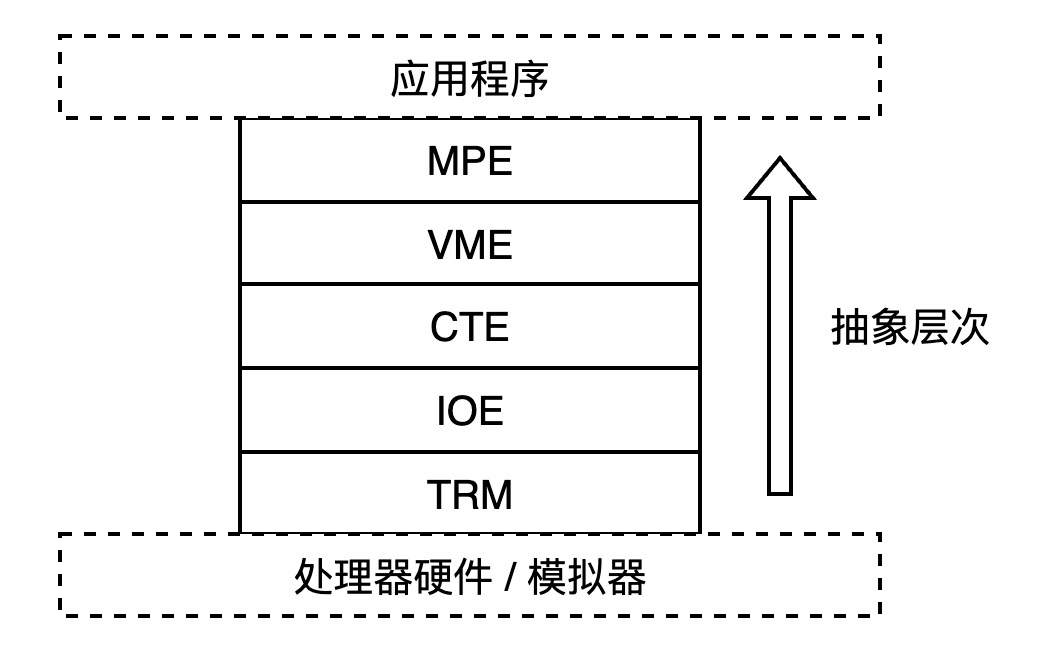
\includegraphics[width=1\linewidth]{assets/13/am-arch.jpg}
  \caption{AM的层次结构}
  \label{fig:am-arch}
\end{figure}

最底层为TRM层，即Turing Machine。
在该层次中，AM提供了一个最简单的、可供计算机进行计算的运行时环境，包括以下功能：

\begin{itemize}
\item
  使用数组\texttt{heap}维护了一块内存空间，即``堆区''，提供给上层程序使用；
\item
  提供了程序入口\texttt{main}，其中包括一个循环；
\item
  提供了程序终止运行的函数\texttt{halt}，上层程序调用该函数即可使其停机；
\item
  提供了打印字符的函数\texttt{putch}。
\end{itemize}

第二层为IOE层，即Input / Output Extension。
该层提供了更多的输入输出方法，例如按格式输出函数\texttt{printf}，以及串口等外设的驱动。
第三层为CTE（Context Extension）层，提供了中断异常的相关服务，完成了上下文的保存恢复工作，并向上层提供了自陷函数\texttt{yield}。
第四层和第五层分别为VME（Virtual Memory Extension）和MPE（Multi-Processor Extension），他们分别实现了虚拟存储和多处理器的相关工作。

在完成AM中全部层次或部分层次的开发后，学生可使用该环境提供的系统服务，编写一些应用程序。
借助南京大学开发的NEMU（NJU Emulator）体系结构模拟器，学生可将自己编写的程序，通过裸机运行时环境AM，运行在体系结构模拟器NEMU上。
其中，学生编写的程序会使用到AM向应用程序提供的系统服务。
在此过程中，学生将对程序运行在计算机上的过程有更深入的理解。

裸机运行时环境AM具有两个特点。
第一，AM将操作系统进行了足够的简化和模块化。
在每个层次中，使用者只需要实现本层次中最基础的功能，即可得到一个具有一定功能的计算机系统，符合敏捷开发流程中对原型开发的重视原则。

第二，AM对计算机系统提供了丰富的抽象层次，层次间互相解耦，因此具有很高的扩展性。
对于其他指令集架构的硬件，AM只需要重构TRM层即可在新的硬件上完成移植。
若要在AM中增加外设，例如增加声卡、网卡，只需要对IOE层进行扩展，提供新的服务函数即可。
因此，使用者可根据需要对AM进行快速增量迭代。

\subsection{在AM上实现极简操作系统}\label{sec:13-operating-system-024}

基于AM的高度层次化和模块化特点，使用者可以使用它开发出系统软件，也就包括操作系统。
在CPU设计结束后，自行设计一套操作系统并且在上面运行，可以打通计算机硬件到计算机软件的整个体系，加深对计算机系统的整体理解。
本节将介绍如何在AM上实现一个简单的操作系统。

为了适配LA32R指令集架构，首先需要将AM的TRM层进行重构。

% 代码语言：BookC
\begin{CodeBlock}[language=BookC]
#include <am.h>
#include <la32r.h>
#include <klib.h>
#include <la32r-csr.h>

extern char _heap_start;
extern char _pmem_end;
int main(const char *args);
void __am_init_uartlite(void);
void __am_uartlite_putchar(char ch);

_Area _heap = {
  .start = &_heap_start,
  .end = &_pmem_end,
};

void _putc(char ch) {
  __am_uartlite_putchar(ch);
}

void _halt(int code) {
  // set $a0 = code
  __asm__ volatile("add.w $r4, %0, $r0" : :"r"(code));
  // syscall 0x11 is nemu trap
  __asm__ volatile("syscall 0x11");

  // should not reach here during simulation
  printf("Exit with code = %d\n", code);

  // should not reach here on FPGA
  while (1);
}

inline void _cache_init()
{
  // invalid icache & dcache, just need two insts due to hardware implementation
  __asm__ __volatile__("cacop 0, $r0, 0" : : : "memory");
  __asm__ __volatile__("cacop 1, $r0, 0" : : : "memory");
}

// dmw0 map va : 0xa0000000 - 0xbfffffff -> pa : 0xa0000000 - 0xbfffffff (SUC PLV0 PLV3)
// dmw1 map va : 0x0 - 0x1fffffff -> pa : 0x0 - 0x1fffffff (CC PLV0 PLV3)
// note that pa : 1fe001e0 - 1fe001d0 has mmio to uart8250 device, so do not use va : 1fe00000 - 1fe0ffff as CC memory!
inline void _dmw_init()
{
  uint32_t dmw0 = 1 | (1 << DMW_PLV3_OFFSET) | (STRONGLY_ORDERED_UNCACHED << DMW_MAT_OFFSET) | (5 << DMW_PSEG_OFFSET) | (5 << DMW_VSEG_OFFSET);
  uint32_t dmw1 = 1 | (1 << DMW_PLV3_OFFSET) | (COHERENT_CACHED << DMW_MAT_OFFSET) | (0 << DMW_PSEG_OFFSET) | (0 << DMW_VSEG_OFFSET);
  csr_write(csr_dmw0, dmw0);
  csr_write(csr_dmw1, dmw1);

  csr_masked_write(csr_crmd, (0 << CRMD_DA_OFFSET) | (1 << CRMD_PG_OFFSET) | (1 << CRMD_DATF_OFFSET) | (1 << CRMD_DATM_OFFSET), CRMD_DA_MASK | CRMD_PG_MASK | CRMD_DATF_MASK | CRMD_DATM_MASK);
}

void _trm_init() {
  __am_init_uartlite();
  _cache_init();
  _dmw_init();
  extern const char __am_mainargs;
  int ret = main(&__am_mainargs);
  _halt(ret);
}
\end{CodeBlock}

在这段代码中，完成了对\texttt{\_heap}的定义，为上层提供了内存区域。在\texttt{\_putc}函数中，使用uart串口打印uart输出。如果希望有其他的输出方式，也可以用其他方法实现\texttt{\_putc}函数。本代码也重写了\texttt{\_halt}函数，作为停止运行的标志，方便进行仿真验证。该函数中进行了系统调用\texttt{syscall\ 0x11}，在仿真验证时，体系结构模拟器NEMU将识别该系统调用，并作为程序运行结束的标志。

由于LA32R架构中，Cache模块的初始化可不由硬件完成，因此在应用程序在待测处理器上运行之前，需要对Cache模块进行清空。上述代码的\texttt{\_cache\_init}函数就完成了该操作，使用LA32R架构规定的\texttt{cacop}指令进行了Cache初始化。

另外，LA32R架构提供了一种特殊的直接映射配置窗口机制。
在处理器处于映射地址模式时，处理器可通过CSR中设置的寄存器直接进行地址翻译，而不通过TLB。
在这段启动代码的编写工作中，也对CSR中的直接映射配置窗口寄存器（\texttt{DMWO},\texttt{DMW1}）进行了配置，从而保证上电后处理器可正常运行程序，即代码中的\texttt{\_dmw\_init}函数。

\texttt{\_trm\_init}是RTM层的顶层函数，将要调用其他函数，以进行环境的初始化工作。

为了方便进行系统的编写，需要对LA32R架构特有的CSR寄存器在代码中进行设置，定义一系列宏，使编程时可直接使用。主要工作是将每个CSR寄存器的每个域进行设置。

% 代码语言：BookC
\begin{CodeBlock}[language=BookC]
#ifndef __LA32RCSR_H__
#define __LA32RCSR_H__

// csr addr define
// copy from regdef.h
#define csr_crmd      0x0
#define csr_prmd      0x1
#define csr_euen      0x2
#define csr_ectl      0x4 // ecfg
#define csr_estat     0x5
#define csr_era       0x6
#define csr_badv      0x7
#define csr_eentry     0xc
#define csr_tlbidx    0x10
#define csr_tlbehi    0x11
#define csr_tlbelo0    0x12
#define csr_tlbelo1    0x13
#define csr_asid      0x18
#define csr_pgdl      0x19
#define csr_pgdh      0x1a
#define csr_pgd       0x1b
#define csr_cpuid    0x20
#define csr_save0     0x30
#define csr_save1     0x31
#define csr_save2     0x32
#define csr_save3     0x33
#define csr_tid       0x40
#define csr_tcfg      0x41
#define csr_tval      0x42
#define csr_ticlr     0x44
#define csr_llbctl    0x60
#define csr_tlbrentry 0x88
#define csr_dmw0      0x180
#define csr_dmw1      0x181

// csr mask define
#define CRMD_PLV_MASK       0x3
#define CRMD_IE_MASK        0x4
#define CRMD_DA_MASK        0x8
#define CRMD_PG_MASK        0x10
#define CRMD_DATF_MASK      0x60
#define CRMD_DATM_MASK      0x180

#define PRMD_PPLV_MASK      0x3
#define PRMD_PIE_MASK       0x4

#define ECFG_LIE_MASK       0x1bff

#define ESTAT_SWI_MASK      0x3
#define ESTAT_HWI_MASK      0x3fc
#define ESTAT_TI_MASK       0x800
#define ESTAT_IPI_MASK      0x1000
#define ESTAT_ECODE_MASK    0x3f0000
#define ESTAT_ESUBCODE_MASK 0x7fc00000

#define LLBCTL_ROLLB_MASK   0x1
#define LLBCTL_WCLLB_MASK   0x2
#define LLBCTL_KLO_MASK     0x4

#define TLBIDX_INDEX_MASK   0xffff
#define TLBIDX_PS_MASK      0x3f000000
#define TLBIDX_NE_MASK      0x80000000

#define TLBELO_V_MASK       0x1
#define TLBELO_D_MASK       0x2
#define TLBELO_PLV_MASK     0xc
#define TLBELO_MAT_MASK     0x30
#define TLBELO_G_MASK       0x40
#define TLBELO_PPN_MASK     0xfffff00

#define ASID_ASID_MASK      0x3ff

#define DMW_PLV0_MASK       0x1
#define DMW_PLV3_MASK       0x8
#define DMW_MAT_MASK        0x30
#define DMW_PSEG_MASK       0xe000000
#define DMW_VSEG_MASK       0xe0000000

#define TCFG_EN_MASK        0x1
#define TCFG_PERIODIC_MASK  0x2
#define TCFG_INITVAL_MASK   0xfffffffc

#define TICLR_CLR_MASK      0x1

// csr field right bits, Indicates how many bits are on the right side of this field
#define CRMD_IE_OFFSET       2
#define CRMD_DA_OFFSET       3
#define CRMD_PG_OFFSET       4
#define CRMD_DATF_OFFSET     5
#define CRMD_DATM_OFFSET     7

#define PRMD_PIE_OFFSET      2

#define ESTAT_ECODE_OFFSET   16
#define ESTAT_ESUBCODE_OFFSET    22

#define LLBCTL_WCLLB_OFFSET  1
#define LLBCTL_KLO_OFFSET    2

#define TLBIDX_PS_OFFSET     24
#define TLBIDX_NE_OFFSET     31

#define TLBEHI_VPPN_OFFSET   13

#define TLBELO_D_OFFSET      1
#define TLBELO_PLV_OFFSET    2
#define TLBELO_MAT_OFFSET    4
#define TLBELO_G_OFFSET      6
#define TLBELO_PPN_OFFSET    8

#define DMW_PLV3_OFFSET      3
#define DMW_MAT_OFFSET       4
#define DMW_PSEG_OFFSET      25
#define DMW_VSEG_OFFSET      29

#define TCFG_PERIODIC_OFFSET 1
#define TCFG_INITVAL_OFFSET  2

// ecode
#define INT_ECODE   0x0
#define PIL_ECODE   0x1
#define PIS_ECODE   0x2
#define PIF_ECODE   0x3
#define PME_ECODE   0x4
#define PPI_ECODE   0x7
#define ADEF_ECODE  0x8
#define ALE_ECODE   0x9
#define SYS_ECODE   0xb
#define BRK_ECODE   0xc
#define INE_ECODE   0xd
#define IPE_ECODE   0xe
#define FPD_ECODE   0xf
#define FPE_ECODE   0x12
#define TLBR_ECODE  0x3f

#define STRONGLY_ORDERED_UNCACHED 0
#define COHERENT_CACHED           1

// csr R/W copy and modify from nexus-am
#define __ASM_STR(x)    #x

// csrrd rd, csr_num
#define csr_read(csr)       \
    ({                      \
        register unsigned int __v;  \
        __asm__ __volatile__("csrrd %0 , " __ASM_STR(csr) \
                            : "=r"(__v)    \
                            :                  \
                            : "memory");       \
        __v;    \
    })

// csrwr rd, csr_num
#define csr_write(csr, val)                                        \
    ({                                                         \
        unsigned int __v = (unsigned int)(val);          \
        __asm__ __volatile__("csrwr %0, " __ASM_STR(csr)  \
                     : "+r"(__v)                           \
                     :                    \
                     : "memory");                  \
    })

// csrxchg rd, rj, csr_num
#define csr_masked_write(csr, val, wmask)                                        \
    ({                                                         \
        unsigned int __v = (unsigned int)(val);          \
        unsigned int __wmask = (unsigned int)(wmask);          \
        __asm__ __volatile__("csrxchg %0, %1, " __ASM_STR(csr)  \
                     : "+r"(__v)                          \
                     : "r"(__wmask)                   \
                     : "memory");                  \
    })

#define TLB_ENTRY_NUM 32

#define tlbsrch() __asm__ __volatile__("tlbsrch": : : "memory")

#define tlbrd() __asm__ __volatile__("tlbrd" : : : "memory")

#define tlbwr() __asm__ __volatile__("tlbwr" : : : "memory")

#define tlbfill() __asm__ __volatile("tlbfill" : : : "memory")

#define invtlb(op, asid, va)                                        \
    ({                                                         \
        unsigned int __asid = (unsigned int)(asid);          \
        unsigned int __va = (unsigned int)(va);          \
        __asm__ __volatile__("invtlb " __ASM_STR(op) ", %0, %1"  \
                     :                            \
                     : "r"(__asid), "r"(__va)                   \
                     : "memory");                  \
    })

#pragma pack(8)
typedef union {
  struct {
    uint32_t E    : 1;
    uint32_t ASID : 10;
    uint32_t G    : 1;
    uint32_t PS   : 6;
    uint32_t VPPN : 19;
    uint32_t      : 27;    
  };
  uint64_t val;
} EntryHi;
#pragma pack()

typedef union {
  struct {
    uint32_t V     : 1;
    uint32_t D     : 1;
    uint32_t MAT   : 2;
    uint32_t PLV   : 2;
    uint32_t PPN   : 24;
    uint32_t pad0  : 2;
  };
  uint32_t val;  
} EntryLo;
\end{CodeBlock}

为了实现操作系统，还需要编写上电后直接运行的程序。在这段程序中，需要对CPU进行进一步的初始化。

% 代码语言：BookLoongArch
\begin{CodeBlock}[language=BookLoongArch]
.section entry, "ax"
.globl _start
.type _start, @function

// start from pc = 0x1c000000
_start:

  // reset cache
  bl _cache_init
  
  // dmw0 map va : 0x0 - 0x1fffffff -> pa : 0x0 - 0x1fffffff (SUC PLV0 PLV3)  for device access
  // dmw1 map va : 0x80000000 - 0x9fffffff -> pa : 0x0 - 0x1fffffff (CC PLV0 PLV3) for memory access
  bl _dmw_init
  
  // set stack pointer to va 0x87000000 (set stack to a higher memory space for _relocate() tempory use)
  ori     $sp, $zero, 0
  lu12i.w $sp, 0x8700
  
  // do relocate, move code and data from spi flash to memory
  bl _relocate

  // jump to memory
  li.w    $t0, 0x80000100
  jirl    $zero, $t0, 0

  .org 0x100

  la.local $sp, _stack_pointer
  bl _trm_init

_excp:
  bl _excp_dispatch
\end{CodeBlock}

这段代码先调用了刚刚定义的\texttt{\_cache\_init}等函数，之后对地址映射窗口进行配置，设置了栈指针，并跳转到\texttt{\_relocate}进行清空工作。之后将跳转到\texttt{\_trm\_init}进行初始化，内部将跳转到程序的运行入口。

还需要编写链接脚本，以保证内存大小等参数正常配置，在链接时进行正确的装载。

% 代码语言：BookLinker
\begin{CodeBlock}[language=BookLinker]
pmem_base = 0x80000000;

OUTPUT_FORMAT(elf32-loongarch);

MEMORY {
  ram (rwxa) : ORIGIN = 0x80000000, LENGTH = 128M
}

INCLUDE "section.ld"
\end{CodeBlock}
